\section{Gravitational Swarm Intelligence}
The Gravitational Swarm Intelligence Algorithm presented in this paper is a modified version of the algorithm presented in the paper "Gravitational Swarm for Graph Coloring" by Israel Carlos Rebollo Ruiz \cite{bib:GravSwarm}. Swarm Intelligence is a model where the emergent collective behavior is the outcome of a process of self-organization, where the agents evolve autonomously following a set of internal rules for their motion, interaction with the environment and the other agents. In this algorithm, the agents are subjected to an environment subject to a version of Newtonian Gravity. Centres of attraction (wells) are placed in the environment and the agents move based upon their attraction to these wells. Each well represents a distinct grouping or colouring of the underlaying graph. Agents experience a repulsive force if they try and enter a well already containing agents that prohibit a valid colouring. If an agent enters a well that is not prohibited, then it stops moving and takes on that well's colour. The algorithm ends once a set iteration limit is reached, or all agents settle into the wells, and hence a valid colouring is found.

\subsection{Implementation and Problems}
The action of each is presented below:
\begin{center}
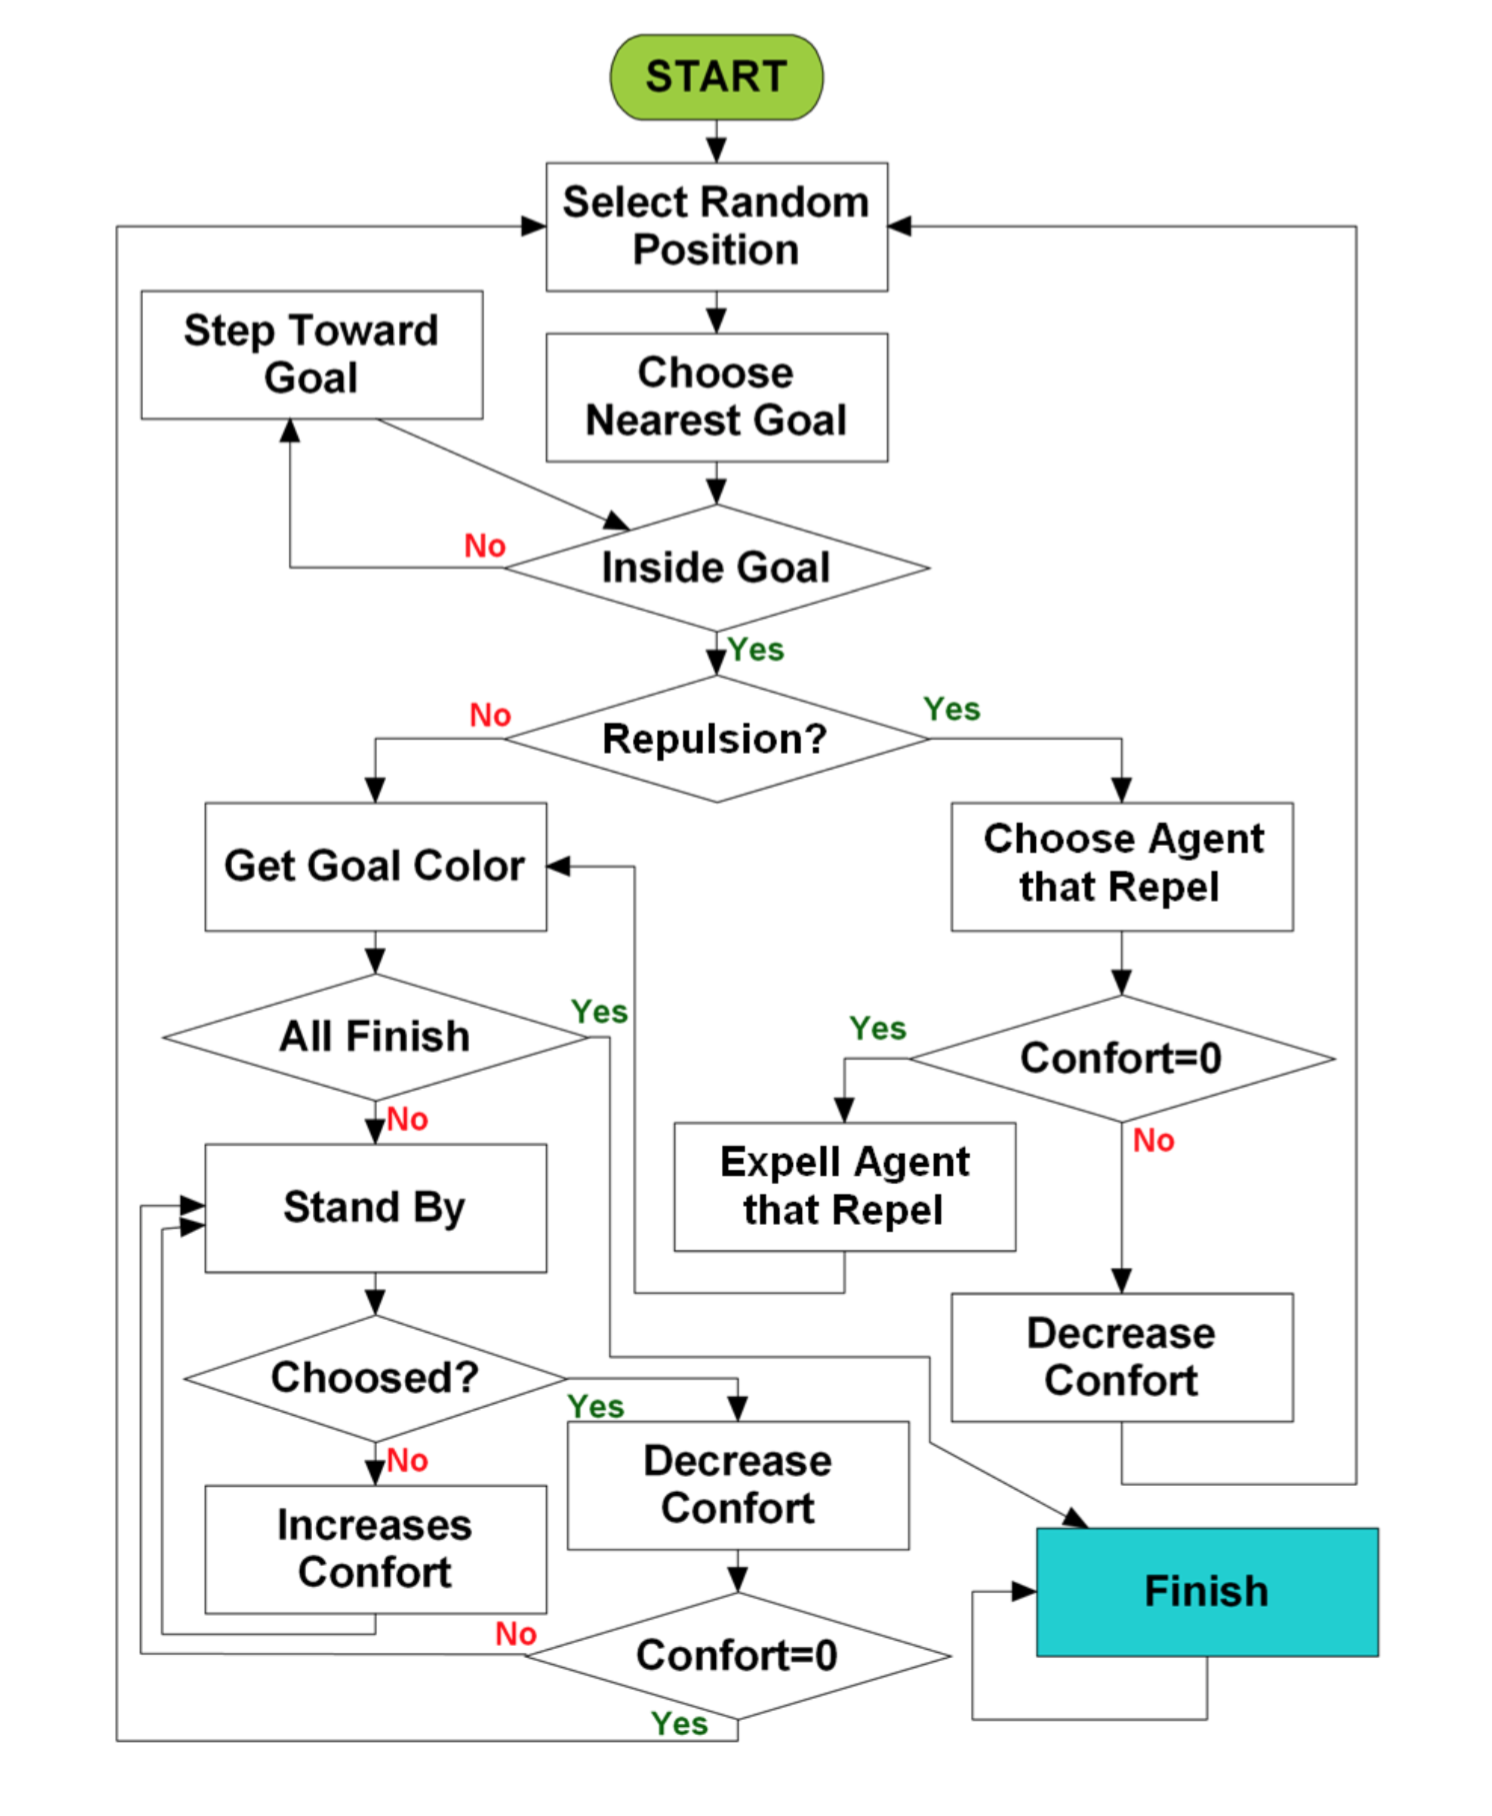
\includegraphics[scale=0.65]{gs-cp-flow}
\end{center}
Each agent moves in the toric world until all agents fall into the "Stand By" State. Then once the last agent triggers the "All Finished" State, the current colouring is accepted as valid. This algorithm presented some issues when implemented for testing. The comfort statistic that each agent tracks can grow unboundedly if the agents repeatedly fall into wells that they are repulsed from. This causes all agents to grow in comfort, making the local minuma harder to improve with every iteration and the chance of jumping out and finding a valid solution fall dramatically. 

\subsection{Workarounds}
\subsection{Additions}